% -*- mode: latex; coding: utf8; TeX-master: algebra-delle-relazioni-massi.tex -*-
% !TeX root = algebra-delle-relazioni-massi.tex
% !TeX encoding = UTF-8 Unicode
% !Tex TS-program = LuaLaTeX
\documentclass[withtimes]{easychair}
\usepackage[utf8]{inputenc}
\usepackage[T1]{fontenc}
\usepackage[italian, english]{babel}
\usepackage[autostyle,italian=guillemets]{csquotes}
\usepackage[backend=biber,style=numeric,hyperref]{biblatex}
\addbibresource{algebra-delle-relazioni-massi.bib}
\usepackage[mode=buildnew]{standalone}% requires -shell-escape
\usepackage{tikz}
\usepackage{caption}
\usepackage{subcaption}
\usepackage{pygmentex}
\usepackage{amsthm}
\usepackage{doc}

\theoremstyle{definition}
\newtheorem{definition}{Definizione}


%% Front Matter
\pagestyle{empty}
\fontfamily{garamond}

\title{Algebra delle Relazioni:\\Un Approccio Pratico alla Teoria delle
Basi di Dati}

\author{
Gionata Massi%\inst{1}\thanks{Ha svolto il ruolo di formatore esperto.}
}

% Institutes for affiliations are also joined by \and,
\institute{
   Istituto di Istruzione Superiore Savoia Benincasa\\
   Ancona, Italia\\
   \email{gionata.massi@savoiabenincasa.it}
}

\authorrunning{Massi}

\titlerunning{Algebra delle Relazioni}

\begin{document}

\maketitle

\selectlanguage{italian}

\begin{abstract}
Questo articolo presenta un approccio pratico all'insegnamento della teoria delle basi di dati relazionali agli studenti delle scuole superiori focalizzandosi sull'algebra delle relazioni. Il corso si rivolge alle classi quarte e quinte del Liceo Scientifico opzione Scienze Applicate, con l'obiettivo di potenziare le competenze STEM e fornire una comprensione  dell'informatica come disciplina scientifica e ingegneristica.

Il percorso didattico di dieci ore introduce i concetti fondamentali delle basi di dati, i Sistemi di Gestione delle Basi di Dati (DBMS) e il \emph{linguaggio SQL}, ponendo particolare enfasi sui principi dell'algebra relazionale e sul loro legame con la logica proposizionale e dei predicati. Il corso utilizza strumenti didattici come una ``calcolatrice'' relazionale online (\emph{RelaX}) e \emph{AlaSQL} per le esercitazioni pratiche in SQL, permettendo una immediata applicazione dei concetti teorici.

Vengono esplorati operatori chiave come \emph{join naturale}, \emph{proiezione}, \emph{restrizione}, \emph{unione} e \emph{differenza insiemistica}, evidenziando le loro corrispondenze logiche e le loro applicazioni pratiche.

L'esperienza ha mostrato che, sebbene l'approccio pratico abbia reso accessibili concetti complessi, la durata  limitata del corso ha impedito l'approfondimento di temi cruciali come la \emph{normalizzazione}. Inoltre, il legame con la \emph{logica formale}, pur essendo intrinseco alla teoria, non è sempre stato pienamente recepito dagli studenti.

Le conclusioni suggeriscono la necessità di rivedere la tempistica e il bilanciamento tra teoria e pratica, e di potenziare gli strumenti didattici per rendere la logica e l'algebra relazionale più intuitive e coinvolgenti.
\end{abstract}

\section{Introduzione}\label{introduzione}

Il corso di dieci incontri da un'ora si propone di introdurre la teoria delle basi di dati relazionali alle classi quarte e quinte del Liceo Scientifico indirizzo Scienze Applicate attraverso un approccio pratico e mirato a rendere i concetti teorici accessibili e direttamente applicabili. Esso rientra nell'ambito del progetto scolastico dell'IIS ``Savoia Benincasa'', ``Citizen scientists of the future'' (C.U.P. H34D23002330006), finanziato dal Piano Nazionale di Ripresa e Resilienza (PNRR), Missione 4 -- Istruzione e Ricerca, Investimento 3.1 ``Nuove competenze e nuovi linguaggi'', con l'obiettivo di potenziare le competenze STEM e multilinguistiche.

Esso introduce alcuni elementi della teoria delle basi di dati relazionali, un pilastro fondamentale dell'informatica come disciplina che studia i metodi per estrarre informazioni in modo automatico da dati grezzi ma strutturati. La presentazione degli argomenti è stata concepita per evidenziare la natura scientifica e ingegneristica dell'informatica,  esponendo sia gli aspetti formali e scientifici (sviluppando l'algebra delle relazioni come estensione della logica dei predicati) sia quelli ingegneristici legati alla rappresentazione (codifiche delle relazioni in tabelle) e all'efficienza computazionale degli algoritmi (semplificazione e ottimizzazione dell'ordine di esecuzione delle \emph{query}). I contenuti si sviluppano in un contesto nel quale la teoria si unisce alla pratica grazie all'utilizzo di una piattaforma web per la valutazione di espressioni algebriche relazionali e alla possibilità di eseguire, via browser, comandi in linguaggio SQL.

Gli obiettivi generali e trasversali includono:

\begin{itemize}
 \item comprendere più a fondo gli oggetti di studio e i metodi della disciplina informatica per poter orientare con maggiore consapevolezza le proprie scelte future (universitarie e professionali);
 \item stimolare l'interesse verso le materie tecnico-scientifiche, in particolare l'informatica;
 \item cogliere la stretta relazione tra pensiero scientifico e sviluppo tecnologico;
 \item comprendere le strutture fondamentali dei ragionamenti logico-deduttivi
e padroneggiare il linguaggio logico-formale.
 \item utilizzare strumenti informatici per modellizzare e risolvere problemi
\end{itemize}

Il corso ricalca in larga parte quello universitario \href{https://www.dcs.warwick.ac.uk/~hugh/#CS252}{CS252.HACD:
\emph{Relational Database Theory}} di Hugh Darwen, e il  materiale didattico è stato progettato a partire da quello realizzato per quel corso: \cite{darwen2014introduction, darwen2010exercises,darwen2011sql}. Si differenzia da esso per il livello, per l'uso della ``calcolatrice'' relazionale online \emph{RelaX}\footnote{La calcolatrice è disponibile all'indirizzo
\url{https://gionata.github.io/relax/calc/local/sb/local/0}). Il fork aggiunge una parziale traduzione in italiano e integra le funzionalità aggiuntive realizzate da Rodrigo Laiola Guimaraes per supportare relazioni di ordine e/o cardinalità zero e migliorare la visualizzazione degli alberi sintattici.} e del \emph{linguaggio SQL} al posto del linguaggio \emph{Tutorial D}.

Gli esempi in linguaggio SQL sono stati realizzati con \href{https://alasql.org/}{\emph{AlaSQL}} e resi disponibili tramite un \href{http://liascript.github.io/course/?https://raw.githubusercontent.com/gionatamassibenincasa/database-didattici/main/algebra_delle_relazioni/README.md}{\emph{open educational resource}} realizzato in \href{https://liascript.github.io/}{\emph{LiaScript}}.

\section{Struttura e Contenuti del Corso}\label{struttura-e-contenuti-del-corso}

Il corso è articolato in moduli progressive, che guidano gli studenti dai concetti introduttivi delle basi di dati ai principi dell'algebra relazionale.

\subsection{Concetti Fondamentali}\label{concetti-fondamentali}

Il percorso inizia esplorando la natura di un database, definendolo come una raccolta \emph{organizzata} di \emph{simboli} interpretabile come un fedele resoconto di un'organizzazione e come una raccolta di \emph{variabili}. Questa sezione introduce anche il concetto di database relazionale, specificando che i suoi simboli sono organizzati in collezioni di relazioni e distinguendo chiaramente il concetto formale di \emph{relazione} dalla sua rappresentazione tabellare (fig.~\ref{fig:variabile}). Vengono poi illustrate le componenti strutturali di una relazione (n-tupla, attributo, grado, cardinalità, intestazione, corpo).

\begin{figure}
    \centering
    \includestandalone[width=.8\textwidth]{img/variabile_relazionale}
    \caption{Variabile relazionale\label{fig:variabile}}
\end{figure}

\subsection{Sistemi di Gestione Database (DBMS) e Linguaggi}\label{sistemi-di-gestione-database-dbms-e-linguaggi}

Si prosegue definendo il \emph{DBMS} come software per la gestione e l'accesso ai database. Viene introdotto il concetto di \emph{linguaggio di database} (o \emph{sottolinguaggio dei dati}), con particolare attenzione al \emph{linguaggio SQL} come strumento per \emph{interrogazioni (query)} e \emph{aggiornamenti delle variabili relazionali}. Il corso illustra le operazioni fondamentali di un DBMS: creazione (\texttt{CREATE\ TABLE}), eliminazione (\texttt{DROP\ TABLE}), gestione di \emph{regole di integrità} (\texttt{PRIMARY\ KEY}, \texttt{FOREIGN\ KEY}, \texttt{CHECK}) e gli \emph{operatori di aggiornamento differenziale} (\texttt{INSERT}, \texttt{DELETE}, \texttt{UPDATE}). L'uso di \href{https://sqlite.org/}{\emph{SQLite}} (tramite  \emph{AlaSQL} e \href{https://it.khanacademy.org/computer-programming/new/sql}{\emph{Khan Academy}}) per la creazione/eliminazione di variabili temporanee è finalizzato all'applicazione pratica dei concetti (fig.~\ref{fig:sql-create-instance}).


\begin{figure}[ht]
  \centering
  \begin{pygmented}[lang=sql]
-- Creazione di una variabile relazionale
CREATE TABLE Iscrizione (
  StudenteId TEXT,
  Nome TEXT,
  CorsoId TEXT,
  PRIMARY KEY(StudenteId, CorsoId)
);
  \end{pygmented}
  \caption{Creazione di una variabile relazionale in SQL}
  \label{fig:sql-create-instance}
\end{figure}


\subsection{Valori, Tipi, Variabili e Operatori}\label{valori-tipi-variabili-e-operatori}

Un modulo dedicato chiarisce le distinzioni essenziali tra \emph{valori} e \emph{variabili}, \emph{tipi} (o \emph{domini}) e \emph{rappresentazioni}
(o \emph{codifiche}), e la natura degli \emph{operatori} (di sola lettura vs.~di aggiornamento, e le loro invocazioni con parametri e argomenti). Viene approfondito il concetto di \emph{tipo} come insieme di valori denominati, la sua funzione nel limitare i valori ammissibili e le specificità della gestione dei tipi (domini) nell'algebra delle relazioni e in \emph{SQLite}. La rappresentazione dei \emph{letterali in SQL} è trattata con esempi pratici. Vengono introdotti gli \emph{Alberi Sintattici Astratti} per la rappresentazione delle operazioni e i \emph{Diagrammi Sintattici} per il linguaggio SQL (fig.~\ref{fig:sql-syntax}). Vengono forniti esempi di espressioni equivalenti e loro visualizzazione come operazione sull'\emph{albero sintattico}.

\begin{figure}[hbt]
    \centering
    \includestandalone[width=.8\textwidth]{img/create_table_syntax}
    \caption{Diagramma sintattico per la creazione di una variabile relazionale in SQL}\label{fig:sql-syntax}
\end{figure}


\subsection{Logica, Proposizioni e Predicati}\label{logica-proposizioni-e-predicati}

Il corso introduce concetti di \emph{logica proposizionale} essenziali per la teoria relazionale. Vengono definiti i \emph{predicati} e la loro relazione con le frasi e le proposizioni che descrivono lo stato del database (fig.~\ref{fig:proposizioni}). Si esplora la \emph{derivazione di predicati da predicati} attraverso l'applicazione di connettivi logici (congiunzione, disgiunzione, negazione, implicazione, bicondizionale) e i \emph{quantificatori} \emph{esistenziale} e \emph{universale}, fornendo le basi logiche per la costruzione delle query e dei vincoli. Vengono inoltre richiamati i concetti fondamentali di \emph{teoria degli insiemi} esprimendoli nei termini della logica dei predicati.


\begin{figure}[htb]
\centering
\begin{tabular}{lclcl}
La studentessa avente matricola & 'S1' & si chiama & 'Anne' & e \\
Lo studente avente matricola & 'S2' & si chiama & 	'Boris'& e \\
La studentessa avente matricola & 'S3' & si chiama & 'Cindy'& e \\
Lo studente avente matricola & 'S4' & si chiama & 'Devinder'& e \\
Lo studente avente matricola & 'S5' & si chiama & 'Boris'&.
\end{tabular}
\caption{Interpretazione della variabile relazionale come congiunzione di proposizioni vere}\label{fig:proposizioni}
\end{figure}

\subsection{Principi di Algebra Relazionale}\label{principi-di-algebra-relazionale}

Questa parte costituisce il cuore teorico-operativo del corso. Si rivisita l'\emph{anatomia di una relazione} e il suo isomorfismo con i predicati. Vengono introdotti gli \emph{operatori dell'algebra relazionale} intesi come operatori logici sulle relazioni:

\begin{itemize}
  \item \textbf{join naturale (\(\bowtie\))}: equivale all'operatore logico AND, con enfasi sulla sua definizione e proprietà. Vengono analizzati i casi particolari (\emph{CROSS JOIN}, o prodotto cartesiano) e le proprietà algebriche.
  \item \textbf{ridenominazione (\(\rho\))}: operatore per rinominare attributi, non presente nella logica dei predicati ma essenziale per estendere il concetto di \emph{join}.
  \item \textbf{equi-join}: viene introdotto come zucchero sintattico per semplificare le espressioni con \emph{join naturale} e \emph{ridenominazione}.
  \item \textbf{Proiezione (\(\pi\))}: corrisponde al quantificatore esistenziale, per determinare l'esistenza di oggetti che soddisfano un predicato.
  \item \textbf{Restrizione (\(\sigma\))} Viene trattato come un caso particolare di \emph{AND} che opera sulle tuple.
  \item \textbf{Estensione}: non presente nella logica, viene introdotto per produrre relazioni con attributi derivati.
  \item \textbf{Operatori di Aggregazione}: introdotti per ridurre ad un valore un insieme di dati (\texttt{SUM}, \texttt{AVG}, \texttt{COUNT}, \texttt{MAX}, \texttt{MIN}), inclusa l'applicazione con \textbf{raggruppamento per (\(\gamma\))}.
  \item \textbf{UNIONE (\(\cup\))}: corrisponde a un OR.
  \item \textbf{DIFFERENZA INSIEMISTICA (\(\setminus\)):} corrisponde ad un \emph{AND NOT}.
\end{itemize}

Ogni operatore è introdotto con la sua definizione formale e esempi pratici, dimostrando come queste operazioni permettano di manipolare e interrogare le basi di dati relazionali (fig.~\ref{fig:table-join}).

Il corso è intervallato da lezioni teoriche e brevi sessioni dedicate agli esercizi. Quelli di logica e di algebra sono fondamentali per consolidare la comprensione dei concetti teorici, mentre quelli in \emph{linguaggio SQL} sono destinati a produrre una conoscenza pratica e applicativa.

\begin{figure}[htp]
	\centering	
	\begin{subfigure}[t]{.75\textwidth}
		\centering
		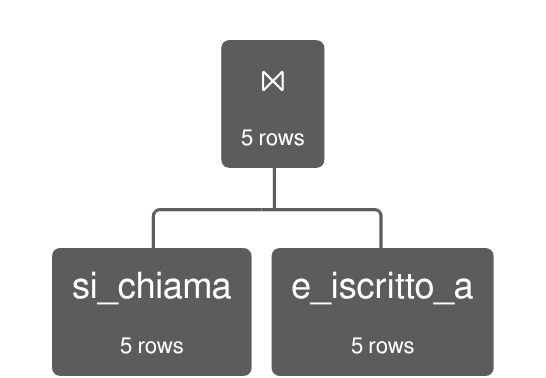
\includegraphics[width=.4\textwidth]{img/inner_join}
		\caption{Albero sintattico del join naturale}\label{fig:inner-join-syn-tree}
	\end{subfigure}

	\vspace{1cm}	
		
	\begin{subfigure}[t]{\textwidth}
		\centering
		\includestandalone[width=.8\textwidth]{img/table_join}
      \caption{Illustrazione del join\label{fig:table-join}}
	\end{subfigure}

	\vspace{1cm}	
	
	\begin{subfigure}[t]{\textwidth}
		\centering
\begin{tabular}{lclclcl}
La studentessa avente matricola & 'S1' & si chiama & 'Anne' & ed è iscritta al corso & 'C1' & e \\
La studentessa avente matricola & 'S1' & si chiama & 'Anne' & ed è iscritta al corso & 'C2' & e \\
Lo studente avente matricola & 'S2' & si chiama & 	'Boris'& ed è iscritto al corso & 'C1' & e \\
La studentessa avente matricola & 'S3' & si chiama & 'Cindy'& ed è iscritta al corso & 'C3' &  e \\
Lo studente avente matricola & 'S4' & si chiama & 'Devinder'& ed è iscritto al corso & 'C1' & . \\
\end{tabular}
\caption{Interpretazione della variabile relazionale come congiunzione di proposizioni vere}\label{fig:proposizioni-join}
	\end{subfigure}
		
	\vspace{1cm}	

	\begin{subfigure}[t]{\textwidth}
		\centering
		\begin{definition}
		Sia $s = r_1 \bowtie r_2$.

Lo schema (intestazione) $H_s$ di $s$ è l'unione delle intestazioni di $r_1$ e $r_2$: $H_s = r_1 \cup r_2$.

Il corpo di $s$ è costituito da quelle tuple con intestazione $H_s$ che possono essere formate prendendo l'unione di $t_1$ e $t_2$, dove $t_1$ è una tupla di $r_1$ e $t_2$ è una tupla di $r_2$.

Se $c$ è un attributo comune, allora deve avere lo stesso tipo dichiarato sia in $r_1$ che in $r_2$. Se non lo ha, allora $r_1 \bowtie r_2$ perde di significato.

Nota: JOIN, come AND, è sia commutativo che associativo.
		\end{definition}
		\caption{Definizione dell'operatore di join\label{fig:join-def}}
	\end{subfigure}

      \caption{Materiale per illustrare l'operatore di join}\label{fig:table-join}
\end{figure}

\section{Conclusioni}\label{conclusioni}

L'esperienza ha evidenziato diverse sfide e opportunità. Sebbene l'approccio pratico abbia contribuito a rendere accessibili concetti complessi, la limitata durata del corso (10 ore) si è rivelata insufficiente per approfondire tutti gli aspetti previsti. In particolare, un tema fondamentale che è rimasto escluso dal corso per limiti di tempo è stato quello della \emph{normalizzazione}. Tempi più distesi avrebbero permesso più attività \emph{hands-on} rispetto alla parte teorica. Inoltre, il \emph{legame con la logica formale}, pur essendo fondamentale per la teoria delle basi di dati e ben immerso nel contesto liceale, non è stato sempre pienamente apprezzato dagli studenti. Sarà necessario rivedere le tempistiche, il bilanciamento tra spiegazioni teoriche e applicazioni pratiche e potenziare gli strumenti per rendere la logica più intuitiva e per superare  limiti dei database estensionali, basati solo su proposizioni vere, a quelli intensionali, che aggiungono regole. Per questo fine si potrebbe aggiungerere in \emph{RelaX} una \emph{interprete} per il linguaggio Datalog, in modo analogo a ``Datalog Educational System\footnote{Un playground del Datalog Educational System è alla url: \url{https://desweb.fdi.ucm.es/}}''\~cite[Saenz-Perez:2011:DDD:1950986.1951133].

\label{sect:bib}
\printbibliography

\end{document}